\documentclass[12pt, a4paper]{report}

\usepackage[spanish]{babel}
\usepackage[utf8]{inputenc}
\usepackage[T1]{fontenc}

\usepackage{enumerate}
\usepackage{eurosym}
\usepackage{graphicx}

\usepackage{hyperref}

\renewcommand*\rmdefault{ptm}
\renewcommand\thesection{\arabic{section}}

\usepackage[a4paper]{geometry}
\usepackage{listings, lstautogobble}
\usepackage{color}

\usepackage{pdfpages}

\definecolor{dkgreen}{rgb}{0,0.6,0}
\definecolor{gray}{rgb}{0.5,0.5,0.5}
\definecolor{mauve}{rgb}{0.58,0,0.82}
\lstset{frame=tb,
  aboveskip=3mm,
  belowskip=3mm,
  showstringspaces=false,
  columns=flexible,
  basicstyle={\small\ttfamily},
  numbers=none,
  numberstyle=\tiny\color{gray},
  keywordstyle=\color{blue},
  commentstyle=\color{dkgreen},
  stringstyle=\color{mauve},
  breaklines=true,
  breakatwhitespace=true,
  tabsize=3,
  autogobble=true
}
\geometry{top=3cm, bottom=3cm, left=3cm, right=3cm}
\graphicspath{ {images/} }

\begin{document}
%----------------------------------------------------------------------------------------
%	TITLE SECTION
%----------------------------------------------------------------------------------------

	\begin{titlepage}
        \raggedleft
        {
        	\Large Universidad de Valladolid \\
        	E.T.S Ingeniería Informática \\
        	Grado en Ingeniería Informática\\
        }
        \vspace{4cm}
        \centering
        {
        	\bf \LARGE Curso 2016/2017 \\
        	 Profesión y Sociedad \\
            
             \vspace{1cm}
        	 Renovarse o morir: \\
             El ciclo de vida de un informático\\
        }
        \vspace{10cm}
        \raggedleft
        {
        	\Large 
            Amigo Alonso, Alberto \\
        	Delgado Álvarez, Sergio \\
            García Prado, Sergio \\
            Iglesias Cortijo, David \\
        }

  \end{titlepage}
  
	\newpage
    \tableofcontents
%----------------------------------------------------------------------------------------
%	TEXT
%----------------------------------------------------------------------------------------

  	\newpage
  	\section{Introducción}
    	\paragraph{}
        La ingeniería informática surgió como la fusión de grandes ámbitos de conocimiento clásicos, como la ingeniería eléctrica, la física o las matemáticas. La combinación de estas ciencias dio lugar a la automatización de trabajos realizados por sistemas computacionales, que mejoraron significantemente la productividad que era conseguida con las anteriores técnicas. Este hecho consiguió atraer la atención de un gran número de investigadores y compañías interesados en desarrollar la potencia de dichos sistemas. 
        
        \paragraph{}
        Desde el primer ordenador Z1 desarrollado por Konrad Zuse, pasando por el ENIAC, UNIVAC, EDSAC y hasta el PDP 11, Spectrum, Apple II o las actuales máquinas Intel se ha desarrollado mucha tecnología en tan solo un siglo \cite{um:historia-infor}. La gran cantidad de disciplinas a las que la computación ha servido para optimizar su proceso productivo (ya sea intelectual o material) ha conseguido que la tecnificación de cada uno de los aportes se haya especializado enormemente. Por ello, actualmente se busca la ubicuidad de los sistemas informáticos en áreas tan diversos como la aviónica, la automoción, la biología o la economía bursátil.
        
        \paragraph{}
        La vertiginosa velocidad con la que se han producido estos avances y la segmentación de sus aplicaciones ha provocado que los profesionales del sector tengan que especializarse en determinados ámbitos. Al tener conocimientos tan específicos para resolver determinado tipo de problemas, se generan problemas para cambiar el enfoque a otras ramas de la informática o simplemente para estar actualizado con las nuevas tendencias y técnicas del sector.
        
        \paragraph{}
        En este trabajo se examinan tanto los sintomas como las soluciones a los problemas creados por este gran progreso en el sector de la informática. El interés del estudio reside en que es completamente innovador, ya que no existe ningún otro que se enfoque en este tema por completo. Por ello, ha implicado la recopilación de información de determinadas fuentes y su sintesis para realizar nuestro propio análisis. Otro gran interés de este trabajo consiste en que, como estudiantes de un grado en ingeniería informática, todos los estudiantes debemos ser conscientes de esta realidad y prepararnos para superarla.
    
    \section{Ciclo de vida de un informático}
    	\paragraph{}
        En este apartado se exponen las etapas generales por las que una persona que se dedique al mundo de las tecnologías de la información y la comunicación suele pasar. Si bien existen casos concretos en los cuales no se siguen dichas etapas, se han identificado estas como generales. Por tanto, se describen más a fondo a continuación, desde el comienzo con el interés por la tecnología hasta la búsqueda de la renovación para no quedarse obsoleto o perder precisamente la motivación adquirida en la primera etapa


    	\subsection{Interés por la tecnología}
        	\paragraph{}
            Es común que hoy en día muchas personas sientan interés por la tecnología, ya sea con fines recreativos o de productividad. Dado que acceder a productos tecnológicos cada vez tiene una barrera económica más baja, hoy en día casi cualquier persona puede acceder a ello. Esto es algo que se contrapone al pasado, donde era mucho más complicado y la principal perspectiva era de mejorar la productividad, sobre todo desde el punto de vista laboral.
            
            \paragraph{}
			Centrándonos más en la perspectiva actual, se exponen las principales vías por las cuáles comienza el interés hacia esta industria. Un hecho a destacar en este punto es que el mayoritariamente surge en edades tempranas, principalmente bajo una perspectiva lúdica. Muchas personas se sienten atraidas por el mundo de los videojuegos, la simplicidad de tareas cuando se realizan con ayuda telemática frente a métodos tradicionales o por la curiosidad de entender cómo se articula la electrónica y el software para conseguir que trabaje un ordenador. 
            
            \paragraph{}
            Si bien las dos primeras vías son un reclamo para muchos de los que terminan dedicandose a ello a nivel profesional, muchas veces el desconocimiento entre el uso y la creación de recursos informáticos es un problema que luego se traduce en fracaso y pérdida del interés en fases siguientes. La conclusión obtenida sobre esta problemática es que está muy condicionada por el desconocimiento debido a la temprana edad de esta disciplina respecto de otras.
 
 
        \subsection{Formación y Obtención de conocimientos}
        
        	\paragraph{}
            La siguiente fase general por la que toda persona que pretenda dedicarse profesionalmente a este sector debe superar es el periodo de formación inicial. La figura \ref{fig:education} muestra un gráfico en el cual se representa el porcentaje de personas que utilizaron cada uno de los mecanismos formativos. Este se ha extraido de la encuesta anual que el sitio web de preguntas y respuestas realiza a personas relacionadas con el sector de las Tecnologías de la Información.
            
             \begin{figure}[htb]
				\centering
				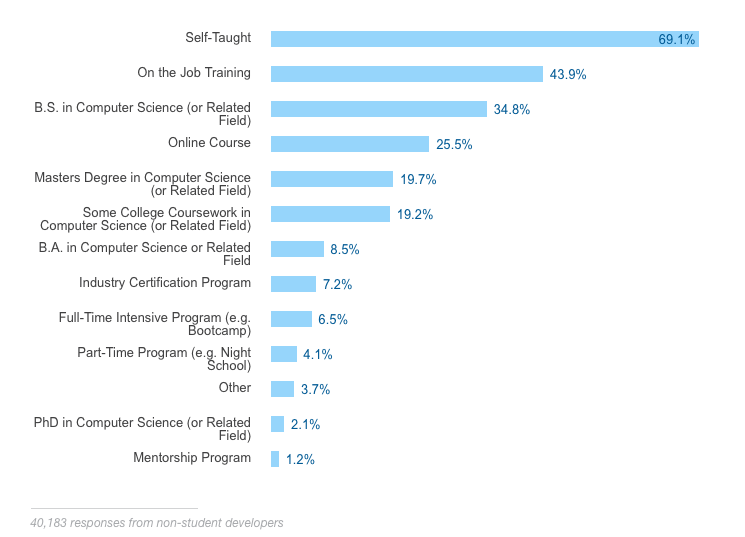
\includegraphics[width=0.8\textwidth]{images/stackoverflow-education}
				\caption{Métodos de aprendizaje más populares.\cite{stackoverflow:survey}} 		
                \label{fig:education}
			\end{figure}  
            
            \paragraph{}
            Debido a que esta etapa tiene muchos posibles caminos y mecanismos, según las perspectivas y objetivos de cada individuo realizaremos una clasificación de las principales alternativas 
            
			\subsubsection{Formación autodidacta}
        		
                \paragraph{}
                Existen muchos casos en el sector de tecnologías de la información en que personas que trabajan en cargos importantes no tienen títulos académicos que abalen su cualificación. La razón de que esto sea así, principalmente es algo derivado de la corta edad del sector. Esto no quiere decir que dichas personas no posean los conocimientos necesarios (posiblemente tengan titulaciones de disciplinas semejantes). Las titulaciones en estudios de Informática no se crean en España hasta la década de los 70.
        	    
                \paragraph{}
                Otro de los detalles importantes por los que hay personas que se deciden por esta alternativa es que el sector en España no está regulado. Lo que se traduce en que para realizar proyectos o actividades que normalmente requerirían de un certificado, debido a los riesgos que implicaría el mal funcionamiento del sistema, no es necesario legalmente poseer ningún tipo de acreditación.
                
                \paragraph{}
				Dejando de lado el tema de las razones por las que escoger esta alternativa, existen muchos recursos para adquirir conocimientos de manera autodidacta, tales como libros, recursos online, documentación específica de determinadas tecnologías, etc. Se comentará más en profundidad el conjunto de recursos disponibles en la sección \ref{subsec:RecursosDisponibles} en la página \pageref{subsec:RecursosDisponibles}.

    		\subsubsection{Formación profesional}
        		
                \paragraph{}
                Las titulaciones de formación profesional en el Sistema Educativo Español se dividen en tres grupos según el nivel de cualificación requerido para su acceso:
                
                \begin{itemize}
					
                    \item \textbf{Programa de Cualificación Profesional Inicial}: 
                    Están orientados a personas sin Educación Secundaria Obligatoria, por lo que sirven para conseguir dicho título junto con la posibilidad de acceder al siguiente nivel de titulación.
                    
                    \item \textbf{Ciclo Formativo de Grado Medio}: 
                    Para acceder a esta titulación es necesario poseer el título de Educación Secundaria Obligatoria. Al finalizar estos estudios se obtiene el título de Técnico en la correspondiente titulación.\cite{wikipedia:fp-spain}
                    
                    \item \textbf{Ciclo Formativo de Grado Superior}:
                   	Se puede optar al acceso de este nivel formativo por diferentes vías: la posesión del título de Bachillerato o de una titulación orientada hacia la misma rama de estudio de un Ciclo Formativo de Grado Medio. finalizar estos estudios se obtiene el título de Técnico Superior en la correspondiente titulación. Terminando estos estudios, posibilitan el acceso a la universidad sin necesidad de hacer la prueba de acceso a la universidad y convalidando créditos en las distintas carreras.\cite{wikipedia:fp-spain}
				
                \end{itemize}

        		\paragraph{}
				Este tipo de titulaciones generalmente están orientadas a la formación en trabajos o tecnologías específicas, por lo que pueden presentar limitaciones a largo plazo. Su duración es de dos cursos lectivos, centrando el último periodo en la realización de prácticas en un entorno laboral que facilite la inserción del titulado al mundo laboral.

        	
    		\subsubsection{Formación universitaria}
        		\paragraph{}
                El siguiente grado de nivel formativo es la titulación universitaria, caracterizada por la adquisición de conceptos fundamentales y generales que luego sirven de base a la hora de entender tecnologías específicas con mayor claridad. Esto tiene limitaciones a corto plazo pero a la vez ventajas a largo plazo. Actualmente este nivel formativo en España se enmarca dentro bajo la visión de Grado, cuya duración es de 4 cursos lectivos, que es equivalente a 240 créditos etcs. Para poder acceder a este tipo de estudios es necesario haber obtenido el título de Bachillerato o poseer una titulación de algún Ciclo Formativo de Grado Superior relacionado con esta rama del conocimiento.
    		   
               \paragraph{}
               Muchas universidades que imparten estudios de informática siguen el documento Computing Curricula, que publica la organización ACM y sirve de guión para plantear los conocimiento que se impartirán. Este texto divide las titulaciones en 5 ramas del conocimiento:
               \begin{itemize}
               		\item \textbf{Ciencias de la Computación}: Abarca un amplio rango de conocimiento, bajo una perspectiva mayoritariamente teórica y de fundamentos algorítmicos hasta el desarrollo de partes criticas en áreas como la robótica, la visión computacional, los sistemas inteligentes, la bioinformática u otras areas novedosas. \cite{acm:computing-curricula}

               		\item \textbf{Ingeniería de Computadores}: Es una disciplina que engloba la ciencia y tecnología del diseño, construción, implementación y mantenimiento de componentes software y hardware de modernos sistemas computacionales y equipamiento controlado por ordenador. \cite{acm:computing-curricula} 

               		\item \textbf{Sistemas de la Información}: Los especialistas en sistemas de información se centran en la integración de soluciones de tecnología de la información y procesos de negocio para satisfacer las necesidades de información de las empresas, lo que les permite alcanzar
sus objetivos de una manera eficaz y eficiente.  \cite{acm:computing-curricula}

               		\item \textbf{Tecnologías de la Información}: es una etiqueta con dos significados. En el sentido más amplio,se usa a menudo para referirse a la totalidad de la informática. En el ámbito académico, se refiere a los programas que preparan a los estudiantes para satisfacer las necesidades de tecnología informática de negocios, gobierno, salud, escuelas y otros tipos de organizaciones. \cite{acm:computing-curricula}

               		\item \textbf{Ingeniería del Software}: Se refiere a la aplicación de un enfoque disciplinado, cuantificable sistemáticamente, para el desarrollo, operación y mantenimiento de software.  \cite{acm:computing-curricula}

               \end{itemize}


            \subsubsection{Formación post-universitaria}
            
        		\paragraph{}
                También existen vías para seguir adquiriendo conocimiento a nivel académico una vez finalizada la formación universitaria. Estas titulación tienen un carácter más especializado en cuanto a la perspectiva bajo la que se imparten. En España se denominan Master, que tiene una duración de entre uno y dos años.
                
                \paragraph{}
				Además, existen programas de Doctorado, generalmente orientados a la investigación. Requieren la superación de una titulación de Master. Tradicionalmente, la concesión de un doctorado implica el reconocimiento de la persona candidata como igual por parte de la facultad de la universidad en la que ha estudiado. Quien obtiene este grado es llamado doctor o doctora.
                


        \subsection{Mundo laboral}
        
        	\paragraph{}
            El periodo laboral se corresponde con la fase más amplia dentro de lo que consideramos ciclo de vida del informático. Es en este periodo cuando se obtiene una remuneración económica por las tareas desempeñadas a la vez que se pone en práctica el conocimiento adquirido en las fases anteriores.
            
            \paragraph{}
            A pesar de la cantidad de campos de especialización dentro del sector, muchas de las tareas requieren realizar un amplio abanico de pasos, que muchas veces son interdisciplinares. Como ejemplo podemos imaginarnos un especialista en bases de datos, al que han pedido la implementación de una determinado alojamiento persistente de información. Para ello dedicará parte de su tiempo tanto a tareas de análisis y codificación de la estructura de la base de datos como a realizar tests o desplegar el sistema. A partir de OpsTalent\cite{opstalent:keep-date} se ha obtenido el gráfico de la figura \ref{fig:time-spend} que muestra los resultados de una estadística sobre la proporción de tiempo que se dedica a cada tarea realizada a personas que trabajan en el sector TI.
           
          	 \begin{figure}[htb]
				\centering
				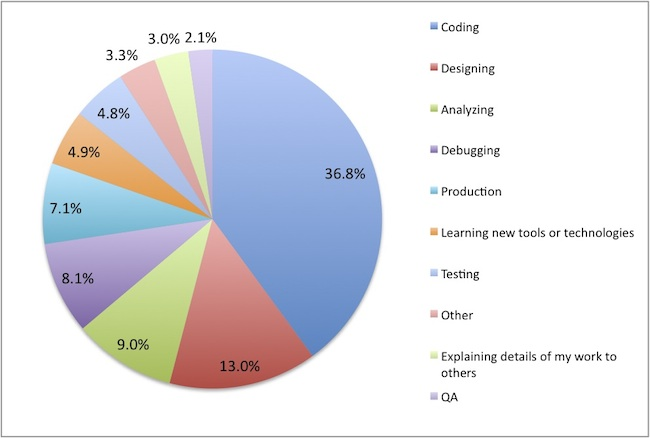
\includegraphics[width=0.8\textwidth]{images/time-spend}
				\caption{Distribución media del tiempo de un informático.\cite{opstalent:keep-date}} 						
                \label{fig:time-spend}
			\end{figure}  
            
            \paragraph{}
            Uno de los puntos a tener en cuenta dentro del mundo laboral es que debe de existir un documento que identifique el conjunto de derechos y deberes a realizar (contrato). Aunque los contratos del sector informático corresponden, en su mayoría, a actos de consumo, también pueden contratarse operaciones complejas de desarrollo de programas específicos o de integración de sistemas que requieren largas negociaciones y una fase precontractual elaborada. Los tipos de contrato más utilizados en el sector son los siguientes: 
            
            \begin{itemize}
            	\item \textbf{Contrato de outsourcing}: Este contrato consiste en la cesión de la gestión de los sistemas de información de una entidad a un tercero que, especializado en esta área del derecho informático, se integra en la toma de decisiones y desarrollo de las aplicaciones y actividades propias de la referida gestión. Su finalidad es la optimizar los resultados de la misma, así como permitir a la entidad el acceso a nuevas tecnologías y la utilización de recursos especializados de los que no dispone. \cite{tuabogadodefensor:contratos}

            	\item \textbf{Contrato de desarrollo}: Una aplicación puede ser una obra creada por encargo, donde el autor se compromete a entregar un software específico, para un determinado uso. Podemos decir que el programa nace de la colaboración entre el proveedor y el cliente ya que es una obra en la que participan tanto el usuario (en la fase de definición de las especificaciones externas) como empresas de servicios o trabajadores independientes. \cite{tuabogadodefensor:contratos}

            	\item \textbf{Contrato de mantenimiento}: Se trata de uno de los contratos informáticos que más se desarrolla en la práctica. La paralización de una empresa por un defectuoso funcionamiento de su sistema informático, produciría enormes pérdidas que, llegado el caso, podrían ser irreparables. De ahí que el empresario ha de contar con un servicio que prevenga este evento o lo corrija en caso que se produzca. \cite{tuabogadodefensor:contratos}

            	\item \textbf{Contrato de auditoria}: Consiste en la revisión de la propia informática y de su entorno. La auditoría informática investiga las instalaciones y los sistemas de tratamiento de la información del empresario o profesional analizando las posibilidades de mejora, detectando fallos en los sistemas, corrigiendo duplicidades, etc. El contrato deberá definir las modalidades según las cuales la empresa consultora realiza, en la sede del cliente, la auditoría general de seguridad de los equipos informáticos en diferentes campos. Dicha auditoría general de seguridad informática exige una colaboración activa entre el auditor y el auditado; el intercambio constante de informaciones tiene por objeto evitar la generación de incidentes perjudiciales. \cite{tuabogadodefensor:contratos}

            	\item \textbf{Contrato de consultoría}: La consultoría consiste en dar asesoramiento o consejo sobre lo que se ha de hacer o cómo llevar adecuadamente una determinada actividad para obtener los fines deseados. El objeto de este acuerdo es el conjunto de actividades necesarias para el estudio y evaluación de los sistemas de información que resulten más adecuados para una empresa determinada. Los contratos de consultoría de software se corresponden normalmente con contratos de servicios, siendo su finalidad la de realizar un estudio o prestar un consejo. 

            \end{itemize}
            
            \paragraph{}
			Las metodologías y maneras de desempeñar las funciones laborales pueden seguir distintos paradigmas, en esta sección se exponen las más populares dentro del sector de las Tecnologías de la Información. Si bien, estas han ido variando su popularidad a lo largo del tiempo, siendo en el pasado el enfoque en Cascada, actualmente están adquiriendo mucha importancia paradigmas metodológicos denominados ágiles (por su facilidad para realizar cambios), que permiten obtener funcionalidad desde fases tempranas. A continuación se exponen en detalle:
            
            \begin{itemize}
				\item \textbf{Modelo en cascada}: Es un proceso secuencial, fácil de desarrollo en el que los pasos de desarrollo son vistos hacia abajo (como en una cascada de agua) a través de las fases de análisis de las necesidades, el diseño, implantación, pruebas (validación), la integración, y mantenimiento. El proyecto está dividido en fases secuenciales. Se hace hincapié en la planificación, los horarios, fechas, presupuestos y ejecución de todo un sistema de una sola vez. Un estricto control se mantiene durante la vida del proyecto a través de la utilización de una amplia documentación escrita, así como a través de comentarios y aprobación por el cliente y la tecnología de la información de gestión al final de la mayoría de las fases, antes de comenzar la próxima fase. \cite{wikipedia:metodologias}

				\item \textbf{Prototipado}: El prototipado permite desarrollar modelos de aplicaciones de software que permiten ver la funcionalidad básica de la misma, sin necesariamente incluir toda la lógica o características del modelo terminado. El prototipado permite al cliente evaluar en forma temprana el producto, e interactuar con los diseñadores y desarrolladores para saber si se está cumpliendo con las expectativas y las funcionalidades acordadas. Los Prototipos no poseen la funcionalidad total del sistema pero si condensa la idea principal del mismo. Paso a Paso crece su funcionalidad, y se maneja un alto grado de participación del usuario. \cite{wikipedia:metodologias}

				\item \textbf{Incremental}: Provee una estrategia para controlar la complejidad y los riesgos, desarrollando una parte del producto software, reservando el resto de aspectos para el futuro. Una serie de mini-cascadas se llevan a cabo, donde todas las fases de la cascada modelo de desarrollo se han completado para una pequeña parte de los sistemas, antes de proceder a la próxima incremental. El concepto inicial de software, análisis de las necesidades, y el diseño de la arquitectura y colectiva básicas se definen utilizando el enfoque de cascada, seguida por iterativo de prototipos, que culmina en la instalación del prototipo final. \cite{wikipedia:metodologias}

				\item \textbf{Espiral}: La atención se centra en la evaluación y reducción del riesgo del proyecto dividiendo el proyecto en segmentos más pequeños para proporcionar más facilidad de cambio durante el proceso de desarrollo, así como ofrecer la oportunidad de evaluar los riesgos y con un peso de la consideración de la continuación del proyecto durante todo el ciclo de vida. Cada viaje alrededor de la espiral atraviesa cuatro cuadrantes básicos: Determinar objetivos, alternativas, y desencadenantes de la iteración, Evaluar alternativas e identificar y resolver los riesgos, Desarrollar y verificar los resultados de la iteración, Planificación de la próxima iteración. Cada ciclo comienza con la identificación de los interesados y sus condiciones de ganancia, y termina con la revisión y examinación. \cite{wikipedia:metodologias}

				\item \textbf{Desarrollo Rápido de Aplicaciones (RAD)}: Es una metodología de desarrollo de software, que implica el desarrollo iterativo y la construcción de prototipos. Intenta reducir el riesgos inherente del proyecto partiéndolo en segmentos más pequeños y proporcionando más facilidad de cambio durante el proceso de desarrollo. Está dedicado a producir sistemas de alta calidad con rapidez, principalmente mediante el uso de iteración por prototipos (en cualquier etapa de desarrollo). Promueve la participación de los usuarios y hace especial hincapié en el cumplimiento de la necesidad comercial, mientras que la ingeniería tecnológica o la excelencia es de menor importancia. La participación activa de los usuarios es imprescindible. Iterativamente realiza la producción de software, en lugar de enfocarse en un prototipo. \cite{wikipedia:metodologias}

			\end{itemize}
            
            \paragraph{}
            Estas metodologías de desarrollo de software siguen en algunos casos, puntos de vista muy diferentes a la hora de abordar un proyecto en la empresa. Además, aunque indirectamente, estas estrategias influencian el sistema organizativo de la organización. Las metodologías en cascada propician estructuras muy jerárquicas y piramidales, que implican la delegación de responsabilidades en el cargo superior. Por contra, otras metodologías como el desarrollo en espiral tienden a generar estructuras más horizontales, en las cuáles se tienen en cuenta en mayor medida las opiniones de todos los empleados, sin importar el puesto que desempeñen en la empresa. 
            
            \paragraph{}
			En el sector de las Tecnologías de la Información el ratio de rotación laboral es muy alto respecto de otros sectores clásicos. Una de las causas por las cuáles sucede esto puede ser el ritmo tan rápido de cambio que experimenta la industria, la cual en muchas ocasiones contrata trabajadores con experiencia en una determinada tecnología para después despedirlos y contratar otros nuevos cuando aparecen otras más novedosas y versátiles. Si bien, las grandes empresas del sector están intentando cambiar esto, tratando de destinar tiempo en el trabajo a que sus empleados se mantengan actualizados para que estos no tengan limitaciones a la hora de trabajar con tecnologías nuevas. 


        	\paragraph{}
            Uno de los datos importantes sobre el mundo laboral es conocer los principales parámetros en los que se fijan los empleados a la hora de seleccionar un empleo frente a otro de características similares. Tal y como se muestra en la figura \ref{fig:job-priorities} extraída de la encuesta realizada por StackOverflow\cite{stackoverflow:survey} podemos saber que el principal motivo es el salario, seguido de indicadores referidos a la calidad  de vida que espera tener el trabajador en la nueva empresa. También cobra mucha importancia el indicador de satisfacción personal correspondiente a las tareas que se espera realizar.
            
             \begin{figure}[htb]
				\centering
				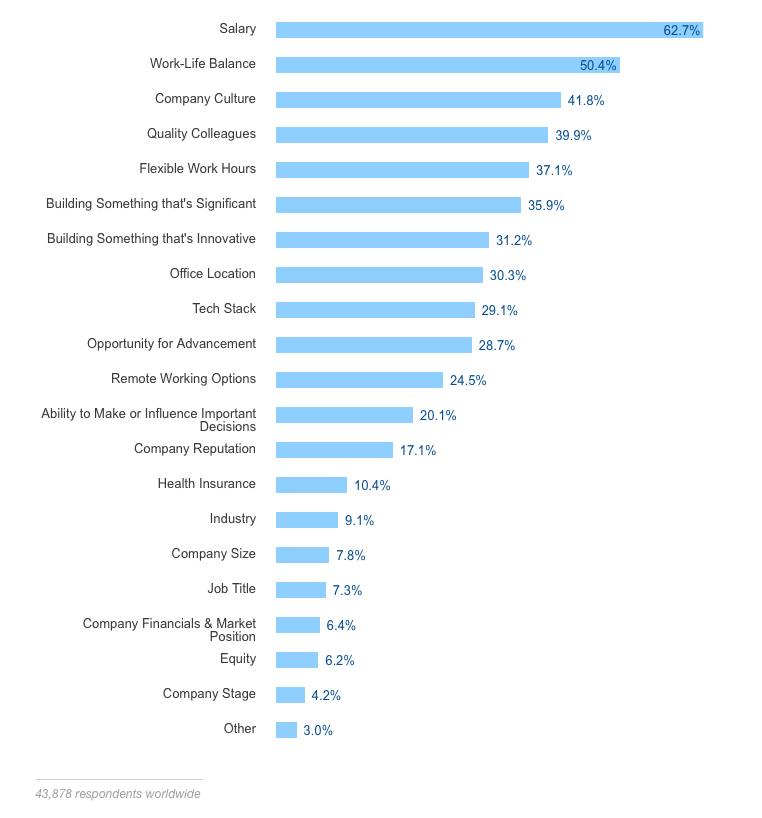
\includegraphics[width=0.8\textwidth]{images/stackoverflow-job-priorities}
				\caption{Métodos de aprendizaje más populares.\cite{stackoverflow:survey}} 		
                \label{fig:job-priorities}
			\end{figure}  
            
                   
        \subsection{Renovación}
        	\paragraph{}
           	El término \emph{renovación} no se refiere a una etapa en concreto que haya que superar, sino más bien es un fenómeno que se debe dar periódicamente durante el periodo de actividad laboral. Dado que este es el tema principal del que habla este artículo en las subsiguientes secciones se expone más en profundidad dicho concepto.
            
    \section{¿Cuándo es necesario renovarse?}
    	\subsection{Situación laboral}
        	\paragraph{}
            La situación laboral es un criterio muy a tener en cuenta para los profesionales a la hora de decidir si deben o no renovarse. Esto es así porque no todos los sectores de la informática evolucionan al mismo ritmo. Como se menciona en el apartado anterior, hay sectores que en los últimos veinte años apenas han avanzado aunque sin embargo, otros han evolucionado enormemente. En los siguientes puntos se trata de aportar una visión sobre algunas de las profesiones que mas se desempeñan en el sector de la informática.
            
             \subsubsection{Desarrollador}
        		\paragraph{}
                ''El desarrollador de software es un programador o una compañía que se dedica a uno o más aspectos del proceso de desarrollo de software. Se trata de un ámbito más amplio de la programación.''\cite{wikipedia:desarrollador}
                
                \paragraph{}
                El desarrollo software es un sector puntero en el ámbito de la informática, y que experimenta una continua y rápida evolución. En los últimos años ha aparecido una gran cantidad de nuevos lenguajes. Aunque las compañías siguen demandando desarrolladores experimentados en lenguajes clásicos tales como Java, C o C++, muchas nuevas organizaciones buscan expertos en nuevos lenguajes como Rust, Go o Swift. En la siguiente gráfica podemos observar como fluctúa el interés de las empresas por algunos de los lenguajes más solicitados.
                
                \begin{figure}[htb]
				\centering
				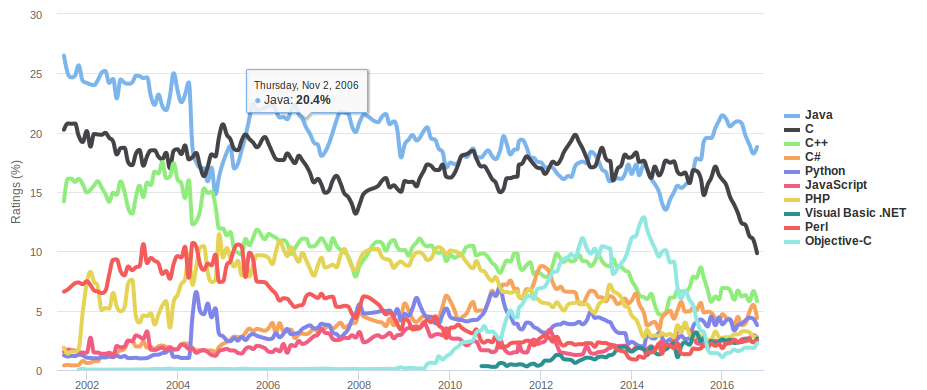
\includegraphics[width=0.8\textwidth]						{images/evolucion_lenguajes}
				\caption{Evolución del interés por los diez lenguajes más solicitados.\cite{tiobe-index}} 		
                \label{fig:leng-evol}
			\end{figure}
            
            Como se observa en esta gráfica lenguajes como Java o C siguen manteniendo su puesto como los lenguajes más solicitados, aunque en la parte baja de la gráfica ocho lenguajes compiten entre sí por un tercer puesto. Esto implica que un profesional en el desarrollo deba estar al tanto de como evoluciona este interés en los diferentes lenguajes y así poder mantenerse dentro del mercado laboral a pesar de esta variación de intereses.
            
    		\subsubsection{Administrador de sistemas}
        		\paragraph{}
                La figura tradicional del admnistrador de sistemas se basa en la implementación, configuración, mantenimiento, monitorización y documentación del correcto funcionamiento de un sistema informático, o algún aspecto de éste. \cite{wikipedia:sysadmin} 
                
                \paragraph{}
                Los conocimientos técnicos de este tipo de profesionales han variado mucho a lo largo del desarrollo de la informática, puesto que los avances en Internet han provocado que los medios de alamacenamiento y de servicios hayan modificado su localidad. También los innovadores sistemas de virtualización han supuesto una alternativa frente a los sitemas clásicos de procesamiento. 
                
                \paragraph{}
                El conocido ''cloud computing'' ha supuesto la mayor migración de conocimiento, ya que ha cambiado el paradigma de proceso de servidores locales de las organizaciones al alquiler de estos recursos localizados en la red. Una empresa puntera en este sector es Amazon con su sistema AWS y EC2. También los sistemas SaaS (Software as a Service) suponen una nueva plataforma de distribución de software que ha de ser dominada por los nuevos administradores. 
                
                \paragraph{}
                En cuanto a la virtualización, supone un ahorro por el mejor aprovechamiento de los recursos existentes en un sistema. Las tecnologías de Vagrant y Docker, entre otras, están siendo las últimas tendencias en este sector.
        	
    		\subsubsection{Profesor e investigador}
        		\paragraph{}
                Dentro del ámbito profesional universitario destacan las figuras del profesor y del investigador, que en muchas ocasiones son ejercidas por la misma persona. Su labor consiste en la divulgación y creación de conocimiento.
                
                \paragraph{}
                Como profesores, se encuentra una gran diferenciación de la necesidad de renovación dependiendo del tipo de asignaturas impartidas. Dentro de áreas de conocimiento que no cambian en gran medida, como los sistemas operativos, las bases de datos o los algoritmos, no resulta necesaria la actualización de conocimientos.
                
                \paragraph{}
                En la faceta de investigadores, los profesionales no necesitan renovarse puesto que son ellos los que están generando el nuevo conocimiento que se aplicará en la industria. Podría entenderse que deben poseer unos solidos conocimientos de estado del arte, pero ello no supone un esfuerzo extraordinario sino que es parte de su trabajo.
                
    	\subsection{Nuevos retos personales}
        	\paragraph{}
            Como en la mayoría de situaciones, en la vida laboral de un trabajador el dinero no supone lo único a tener en cuenta. Esto produce una necesidad a un profesional obsoleto de actualizar sus competencias o incluso ir más allá, solo por evitar quedarse atrás en un mundo que evoluciona a un ritmo frenético.
            
            \paragraph{}
			El que un profesional se sienta estancado en su puesto de trabajo porque lleva años haciendo lo mismo o porque su puesto se ve amenazado por gente más joven que acaba de concluir sus estudios de grado, produce una insatisfacción muy grande en el trabajador. Una solución podría ser optar por actualizar sus conocimientos dentro de su ámbito profesional o incluso aventurarse a explorar otros campos de la informática ligeramente diferentes al suyo.

			\paragraph{}
			El aumento de conocimientos por parte de un trabajador produce una repercusión muy positiva en él mismo, ofreciéndole la oportunidad de acceder a cargos superiores dentro de su propia empresa, afectando beneficiosamente a su remuneración económica e incluso a su calidad de vida y satisfacciones personales.
			
            \paragraph{}
			Otro de los motivos que pueden alentar a un profesional a actualizarse o buscar nuevas competencias, es la decisión de utilizar sus habilidades en favor del bien público. Por ejemplo en el caso de un investigador TIC que llegado un momento de su vida profesional quiere dar un vuelco a su campo y dedicarse a tecnologías aplicadas a la medicina.

			\paragraph{}
			En conclusión, no solo la situación laboral repercute en la necesidad personal de actualizar los conocimientos de un profesional, sino que hay motivos que pueden llegar a ser incluso mas importantes que la obsolescencia dentro de un puesto de trabajo.

		\subsection{Ritmo de evolución en el sector}
        	\paragraph{}
			La informática es un sector que evoluciona a un ritmo vertiginoso, lo que implica que los expertos en el sector tengan que adaptarse a este ritmo de avances y evolucionar junto a ella. Es decir, deben renovarse.
            
            \paragraph{}
           	Hace unos años, cuando la informática comenzaba su auge, era sencillo mantenerse al corriente de los diferentes aspectos de la informática, ya que existía, por ejemplo, un libro de referencia para las bases de datos, otro para los sistemas operativos, etcetera. Hoy en día es prácticamente imposible estar al tanto de todos estos aspectos, ya que hay tal volumen de información que se amplía día a día, que es difícil contrastarla y seleccionarla para su posterior estudio.
        	
            \paragraph{}
            Este ritmo de evolución ha provocado la ramificación de la informática en diversas disciplinas, que abarcan diferentes áreas de conocimiento. Como observamos en la figura (\ref{fig:disciplina}), antes de los años noventa la informática estaba dividida en dos disciplinas: la Ingeniería de Computadoras(CE) y los Sistemas de Información(IS). Después de los años noventa aparecen tres nuevas disciplinas: Ciencias de la computación(CS), Ingeniería del Software(SE) y Tecnologías de la Información(TI). Estas cinco disciplinas definen las áreas de conocimiento de la informática en la actualidad.
            
            \begin{figure}[htb]
				\centering
				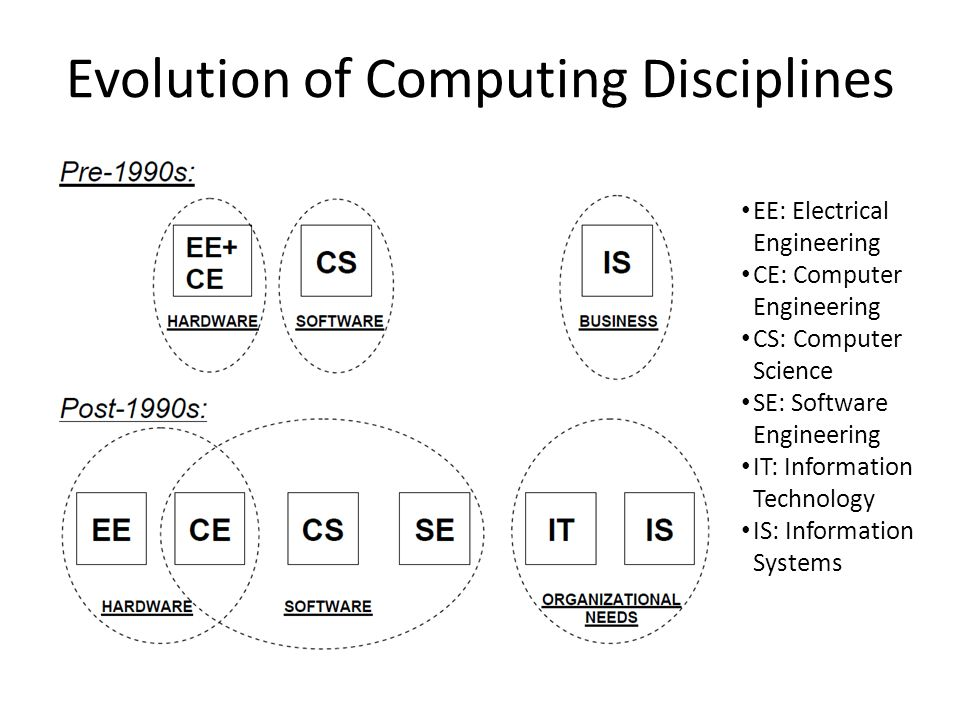
\includegraphics[width=0.8\textwidth]{images/disciplines.jpg}
				\caption{Disciplinas de la informática según la ACM.} 						
                \label{fig:disciplina}
			\end{figure}
			
            \paragraph{}
            Esta ramificación, permite en cierta medida renovarse a los informáticos, ya que solo deberán transformar los conocimientos en la disciplina en la que se haya especializado. 
            
            \paragraph{}
            Esta evolución no afecta únicamente al sector de la informática, sino que  otras disciplinas como la medicina o la ingeniería industrial también se ven afectadas por la evolución en sus respectivas áreas de conocimiento. El factor fundamental que marca la diferencia en la importancia de renovarse entre estas disciplinas y la informática es el ritmo de evolución, ya que en las últimas décadas la informática esta siendo el centro de atención en los ámbitos económicos, sociales, laborales, etcetera. Esto provoca una demanda por parte de los consumidores que obliga a este sector a estar en rápida y continua evolución, a diferencia de otras disciplinas que, aunque siguen evolucionando no están en su momento de auge, ya sea porque tuvieron una temprana aparición como la medicina o simplemente porque no están en el centro de atención.           
            
    \section{El proceso de renovación}
    
    	\subsection{Recursos disponibles}
        \label{subsec:RecursosDisponibles}

    		\paragraph{} 
            A medida que el mundo de la informática evoluciona, aumenta la cantidad de recursos existentes para adquirir nuevos conocimientos y actualizar aquellos ya adquiridos. Con la creación de las últimas ramas y la especialización de las teorías existentes, cada vez se distribuye mas el conocimiento en diferentes recursos que puedan abarcar el contenido por completo. A continuación se exponen los principales tipos de recursos que están a disposición de los usuarios.
            
        	\subsubsection{Libros}
        		\paragraph{} 
				Existe una cantidad abundante de bibliografía para aquellos profesionales que quieran actualizar sus conocimientos, de tal manera que con tener acceso a bibliotecas especializadas se puede cubrir todas aquellas necesidades de conocimiento que este ritmo de evolución pudiera ocasionar.
                
                \paragraph{}
            	Las últimas actualizaciones de las materias suelen presentarse en los artículos de investigación publicados por los investigadores en lugar de en los libros de texto. Por ello es extremadamente recomendable el conocimiento de los congresos científicos relevantes asociados al sector.
                
    		\subsubsection{Cursos}
        		\paragraph{}
               	Otra de las formas existentes para poder adquirir nuevas competencias que ayuden al informático a mantenerse activo y actualizado en su sector son los cursos de formación.
                
                \paragraph{}
                Actualmente muchas universidades imparten cursos enfocados en conocimientos concretos dentro del mundo de la informática. La realización de estos cursos ayuda a aquellos informáticos que estén desactualizados a adquirir la capacidad de poder realizar su trabajo con conocimiento de las innovaciones tecnológicas de su campo. Este tipo de cursos se presentan en forma de Másteres universitarios o promovidos por las fundaciones de las universidades como las de la FunGe de la Universidad de Valladolid, por ejemplo.
                
                \paragraph{}
				Una de las fuentes de cursos mas importantes son las empresas relacionadas con el mundo de la informática, que además ofertan certificaciones muy valoradas en el ámbito laboral. Es el caso de CISCO en lo referido a certificaciones para administradores de redes, o Microsoft, que oferta cursos con certificación para la mayoría de sus productos\cite{microsoft:cursos}.
        	
    		\subsubsection{Recursos online}
        		\paragraph{}
        		Existe una cantidad muy grande de recursos en línea sobre los conocimientos tecnológicos más actualizados, aunque el mayor de los problemas de esta información es que no todos aquellos conocimientos provienen de fuentes fiables. Los recursos online son utilizados sobre todo por las personas autodidactas, aquellas personas que utilicen este método de aprendizaje y actualización de sus competencias deberá procurar que la información que consulten es recomendable que esté firmada por instituciones o personas de renombre en el mundo de la informática o universidades especializadas.
            
    		\subsubsection{Vuelta a la universidad}
        		\paragraph{}
        		A pesar de que no es una costumbre muy popular en España, en otros países existe un flujo constante de entrada y salida entre la universidad y el mundo laboral. Las personas que acaban sus estudios de grado acostumbran a entrar al mundo laboral, para unos años después regresar a la universidad y así continuar sus estudios realizando algún máster especializado, continuando con este proceso a lo largo de su vida activa como informáticos.
        
                
    \section{Conclusiones}
    	\paragraph{}
        Seguramente muchos profesionales pensarán que renovarse es algo innecesario y posiblemente en algunos casos tengan razón. Hay ciertos campos de la informática que no han evolucionado demasiado en los últimos veinte años, pero en la mayoría, el crecimiento y la evolución ha sido abismal. Muchos ingenieros que han estado desconectados de gran parte de la evolución de la informática desconocerán términos como Azure, Spark o BigData entre otras competencias tecnológicas de las más solicitadas en la actualidad\cite{universia:competencias}.
        
        \paragraph{}
        Este desconocimiento en los campos más novedosos y demandados puede ocasionar un desnivel entre ingenieros desactualizados, los nuevos ingenieros que entran a trabajar en una empresa y aquellos ingenieros que hayan estado reciclando sus conocimientos. Quedando atrás a aquellos profesionales que hayan decidido no renovarse, incluso pudiendo llegar a perder su puesto de trabajo en el caso de que sus conocimientos no se adapten a las necesidades de la organización.
        
        \paragraph{}
        Debido a la problemática de no renovarse, muchas empresas apuestan por la renovación de los conocimientos de sus empleados, a través de cursos formativos complementarios. Esto les permite ampliar sus aptitudes profesionales acorde con el ritmo de evolución del sector. Proporcionando un beneficio para la organización, ya que se pierde la necesidad de contratar nuevo personal con conocimientos más actuales. En contrapartida, otras organizaciones prefieren no hacerse cargo de estos costes formativos complementarios para sus trabajadores. Por lo tanto buscaran profesionales capaces de mantener sus conocimientos y aptitudes profesionales actualizadas.
        
        \paragraph{}
       	Nuestra perspectiva acerca de dicha problemática es que conforme pase el tiempo, el sector de la informática tenderá a estabilizarse, por lo que estos problemas tendrán consecuencias menos graves en el futuro.
        
        
%----------------------------------------------------------------------------------------
%	Bibliographic references
%----------------------------------------------------------------------------------------
	\begin{thebibliography}{9}
    
        \bibitem{um:historia-infor}
        Universidad de Murcia: Historia de la informática \url{http://www.um.es/docencia/barzana/IATS/Iats04.html}
        
        \bibitem{stackoverflow:survey}
        StackOverflow: Developer Survey 2016 \url{http://stackoverflow.com/research/developer-survey-2016}
        
		\bibitem{wikipedia:fp-spain}
		Wikipedia: Formación profesional en España. \url{https://es.wikipedia.org/wiki/Formación_profesional_en_España}
        
        \bibitem{acm:computing-curricula}
        ACM: Computing Curricula. \url{http://www.acm.org/education/curricula-recommendations}
        
        \bibitem{opstalent:keep-date}
        Opstalent: Developers need to keep date latest technologies time. \url{http://www.opstalent.com/developers-need-keep-date-latest-technologies-time}
        
        \bibitem{wikipedia:metodologias}
		Wikipedia: Metodología de Desarrollo Software. \url{https://es.wikipedia.org/wiki/Metodologia_de_desarrollo_de_software}
        
         \bibitem{wikipedia:desarrollador}
		Wikipedia: Desarrollador Software. \url{https://es.wikipedia.org/wiki/Desarrollador_de_software}
        
        \bibitem{wikipedia:sysadmin}
        Wikipedia: Administrador de sistemas \url{https://es.wikipedia.org/wiki/Administrador_de_sistemas}
        
        \bibitem{tiobe-index}
		Tiobe: Estudio de la evolución del interes de los lenguajes de programación por las empresas. \url{http://www.tiobe.com/tiobe-index/}
        
         \bibitem{microsoft:cursos}
		Microsoft: Cursos de infromática para productos y teconologías Microsoft. \url{https://www.microsoft.com/es-es/learning/}
        
        \bibitem{universia:competencias}
		Universia: Competencias tecnológicas demandadas por las empresas. \url{http://noticias.universia.pr/practicas-empleo/noticia/2016/05/03/1138945/8-habilidades-tecnologicas-demandadas.html}
        
         \bibitem{tuabogadodefensor:contratos}
		Tu Abogado Defensor: Contratos informáticos. \url{http://www.tuabogadodefensor.com/contratos-informaticos/}
        
        
        
	\end{thebibliography}
  
\end{document}


